\documentclass{asaproc}

\usepackage{dsfont}
\usepackage{graphicx}
\usepackage{bm}
\newcommand{\m}[1]{\mathbf{\bm{#1}}}
\newcommand{\R}{I\hspace{-4.4pt}R}

%\usepackage{times}
%If you have times installed on your system, please
%uncomment the line above

%For figures and tables to stretch across two columns
%use \begin{figure*} \end{figure*} and
%\begin{table*}\end{table*}
% please place figures & tables as close as possible
% to text references


\newcommand{\be}{\begin{equation}}
\newcommand{\ee}{\end{equation}}

\title{Models for Mount Etna interevent times}

%input all authors' names

\author{Mickey Warner \\ AMS 207 Midterm Exam}

%input affiliations

%{USDA Forest Service Forest Products Laboratory}

\begin{document}

\maketitle


\begin{abstract}
Located on the east coast of Sicily, Italy, Mount Etna is an active volcano and as such there is an interest in estimating the time until the next eruption. For just over four centuries, the dates of eruptions have been recorded allowing us the easy calculation for number of days between eruptions, termed interevent time. We present and compare two models for the log interevent times.
\end{abstract}

\section{Introduction}
Interevent times measure the number of days between eruptions for Mount Etna. Across four hundred years, 62 events took place. Some events occurred as little as 40 days apart, while several happened over 10 (and in one case 53) years after the previous eruption. This right-skewness leads us to take the logarithm of the interevent times (Figure \ref{data}). The histogram for the data seems to suggest normality. However, we still expect long tails, leading us to consider two models: (1) a student-$t$ with random effects for the location, and (2) a normal distribution.

We present the details of the two models in section 2, the sampling scheme to obtain posterior draws, and the methods for validating and comparing the two models. In section 3 we report an analysis of the models. We concluded with a discussion in section 4.
\begin{figure}[ht]
\centering
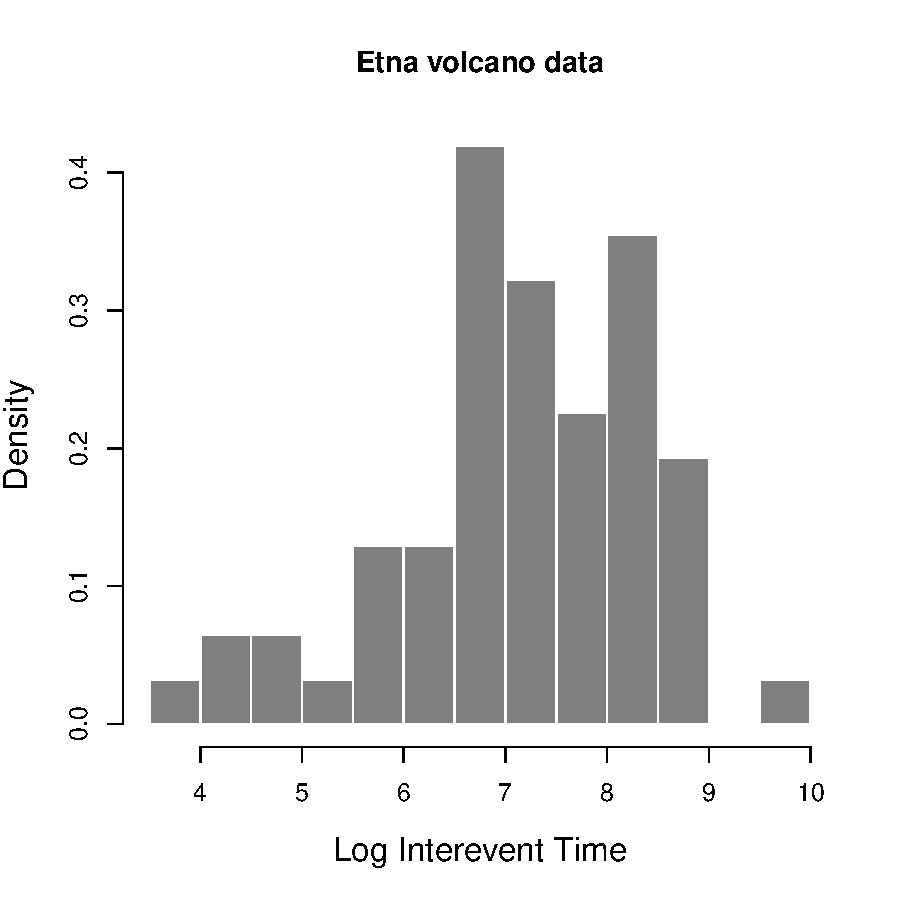
\includegraphics[scale=0.55]{figs/data.pdf}
\caption{Histogram for the $n=62$ log interevent times.}
\label{data}
\end{figure}

\section{Methods}

For both models, define $Y_i=\log T_i$, where $T_i$ is the interevent time for the $i$th observation.

\subsection{Model 1: Student-$t$ (M1)}

In order to better model the long tails we expect in the data, we assume a student-$t$ likelihood where each of the $n=62$ observations receives its own random effect:
\begin{eqnarray*}
y_i|\mu_i,\sigma^2 &\sim& t_\nu(\mu_i, \sigma^2),~~~~~i=1,\ldots,n \\
\mu_i|\mu,\tau^2 &\sim& N(\mu, \tau^2),~~~~~i=1,\ldots,n
\end{eqnarray*}
We fix $\nu=5$. After choosing priors for $\mu$, $\sigma^2$, and $\tau^2$ we could sample from the posterior using Metropolis updates. Alternatively, we could use the definition for the $t$ distribution as a scale mixture of normals enabling us to obtain closed-form full posterior conditionals. That is,
\begin{eqnarray*}
f(y_i|\mu_i,\sigma^2) = \int_0^\infty N\left(y_i|\mu_i, \frac{\sigma^2}{\lambda_i}\right)Ga\left(\lambda_i|\frac{\nu}{2},\frac{\nu}{2}\right)d\lambda_i.
\end{eqnarray*}
This implies the following model
\begin{eqnarray*}
y_i|\mu_i,\sigma^2,\lambda_i &\sim& N(\mu_i, \sigma^2/\lambda_i), \\
\lambda_i &\sim& Ga(\nu/2, \nu/2), \\
\mu_i|\mu,\tau^2 &\sim& N(\mu, \tau^2).
\end{eqnarray*}

Choosing a normal prior for $\mu$ and inverse gamma priors for $\sigma^2$ and $\tau^2$ completes the model formulation:
\begin{eqnarray*}
\mu &\sim& N(m, s^2), \\
\sigma^2 &\sim& IG(a_\sigma, b_\sigma), \\
\tau^2 &\sim& IG(a_\tau, b_\tau).
\end{eqnarray*}

It is straightforward to obtain the full conditionals for each parameter. They are given by
\begin{eqnarray*}
\lambda_i|\cdot &\sim& Ga\left(\frac{\nu+1}{2}, \frac{\nu}{2}+\frac{1}{2\sigma^2}(y_i-\mu_i)^2\right), \\
\mu_i|\cdot &\sim& N\left(\frac{\tau^2y_i\lambda_i+\sigma^2\mu}{\tau^2\lambda_i+\sigma^2},\frac{\tau^2\sigma^2}{\tau^2\lambda_i+\sigma^2}\right), \\
\mu|\cdot &\sim& N\left(\frac{s^2\sum_{i=1}^n\mu_i+\tau^2m}{ns^2+\tau^2},\frac{s^2\tau^2}{ns^2+\tau^2}\right), \\
\sigma^2|\cdot &\sim& IG\left(a_\sigma+\frac{n}{2},b_\sigma+\frac{1}{2}\sum_{i=1}^n\lambda_i(y_i-\mu_i)^2\right), \\
\tau^2|\cdot &\sim& IG\left(a_\tau+\frac{n}{2},b_\tau+\frac{1}{2}\sum_{i=1}^n(\mu_i-\mu)^2\right).
\end{eqnarray*}
We are assuming prior independence among all of the variables. This may not be realistic, particularly for the joints of mean and variance parameters, but we are left with a posterior that is easy to work with. Also, we have not consulted expert opinion to help identify any prior dependence. Consequently, we choose somewhat non-informative values for $m$, $s^2$, $a_\sigma$, $b_\sigma$, $a_\tau$, and $b_\tau$. We choose $m=6$ which corresponds to a prior average interevent time of $\exp(6)=403~\mathrm{days} \approx 1~\mathrm{year}$. $s^2=10$ is very non-informative, especially on the log-scale. We let  $a_\sigma=a_\tau=3$ and $b_\sigma=b_\tau=4$ which yield prior means of $2$ and variances of $4$ for both $\sigma^2$ and $\tau^2$.

\subsection{Model 2: Normal (M2)}

A much simpler model is also considered:
\begin{eqnarray*}
y_i|\mu,\sigma^2 &\sim& N(\mu, \sigma^2),~~~~~i=1,\ldots,n \\
\mu &\sim& N(m, s^2), \\
\sigma^2 &\sim& IG(a_\sigma, b_\sigma).
\end{eqnarray*}
We use the same values for $m$, $s^2$, $a_\sigma$, and $b_\sigma$ from above. The full conditionals are given by
\begin{eqnarray*}
\mu|\cdot &\sim& N\left(\frac{s^2\sum_{i=1}^ny_i+\sigma^2m}{ns^2+\sigma^2},\frac{s^2\sigma^2}{ns^2+\sigma^2}\right), \\
\sigma^2|\cdot &\sim& IG\left(a_\sigma+\frac{n}{2},b_\sigma+\frac{1}{2}\sum_{i=1}^n(y_i-\mu)^2\right). \\
\end{eqnarray*}

\subsection{Model validation and comparison}

\subsubsection{Validation}

We utilize two measures for model fit. The first is a $\chi^2$ test from Johnson (2004) in ``A Bayesian $\chi^2$ Test for Goodness-of-Fit.'' The test is comparable to classical $\chi^2$ goodness-of-fit tests. With this test, we calculate a distribution of $p$-values where high values are in favor of a good model fit. See Johnson (2004) for details.

The second measure is based on leave-one-out cross-validation. We obtain $B$ posterior draws for each model while leaving one observation out, $y_i$. Posterior predictions $y_{j,b}^*$ are then obtained and we compute
\begin{eqnarray*}
p_{j,i}=\frac{1}{B}\sum_{b=1}^B \mathds{1}(y_{j,b}^* \leq y_i),~~~~~j=1,2
\end{eqnarray*}
Distribution theory requires that $p_{j,\cdot}$ be uniformly distributed for the model to be appropriate. The Kolmogorov-Smirnov test is used to determine whether $p_{j,\cdot}$ is uniform.

Graphically, a kernel density plot of the posterior predictive distribution against the data can provide a quick assessment for the model fit.

\subsubsection{Comparison}

To compare models 1 and 2, we use three measures. The deviance information criterion (DIC) is defined as
\begin{eqnarray*}
DIC=\bar{D}(\theta)+\widehat{\mathrm{var}}(D(\theta))/2
\end{eqnarray*}
where $D(\theta)=-2\log p(\m{y}|\theta)$, $\bar{D}(\theta)$ is the average of $D(\theta)$ over all posterior samples $\theta$ and $\widehat{\mathrm{var}}(D(\theta))$ is the sample variance of $D(\theta)$. DIC measures goodness-of-fit and penalizes model complexity; a lower DIC is preferred.

The second measure is the posterior predictive loss (PPL) which is similar in nature to DIC. It is computed by
\begin{eqnarray*}
PPL=G+P=\sum_{i=1}^n(y_i-\mu_i^*)^2 + \sum_{i=1}\sigma_i^*
\end{eqnarray*}
where $\mu_i^*$ and $\sigma_i^*$ are the mean and variance of the posterior prediction for observation $i$.

The third and final measure we use is the Bayes factor. The Bayes factor in favor of model 1 is given by
\begin{eqnarray*}
B_{12}=\frac{\int_{\Theta_1}p_1(\m{y}|\theta)g_1(\theta)d\theta}{\int_{\Theta_2}p_2(\m{y}|\theta)g_2(\theta)d\theta} = \frac{m_1(\m{y})}{m_2(\m{y})}
\end{eqnarray*}
Large values of $B_{12}$ give evidence in favor of model 1. We do not evaluate either integral. Instead, we estimate $m_j(\m{y})$ using Monte Carlo integration. By sampling $N$ times from the prior for model $j$, we can obtain the approximation
\begin{eqnarray*}
m_j(\m{y})=E_{g_j}[p_j(\m{y}|\theta)] \approx \frac{1}{N}\sum_{i=1}^Np_j(\m{y}|\theta_i),~~~~~j=1,2
\end{eqnarray*}
An immediate drawback to this approach is the instability of the estimate. We have to choose $N$ very large to get a somewhat believable Bayes factor, but even then we are not as confident in using this measure over the first two.

\section{Results}

Posterior draws for models 1 and 2 are obtained by iteratively sampling from the full conditionals as given in sections 2.1 and 2.2. We obtain $B=20000$ draws and did not observe any issue with the sampler to be concerned with convergence. Some of the posterior distributions are presented in Figure \ref{m_post}.  In each figure, red figures and objects correspond to model 1 while blue is reserved for model 2.

Since model 1 is hierarchical, there are several ways to obtain posterior predictions. We could make predictions for observation $i$, given the posterior draws for $\mu_i$, $\sigma^2$, and $\lambda_i$. Figure \ref{obs_fit} shows a plot of the observed versus the fitted values for each observation. Note the trends in the figure. The mean predictions (the dots) are systematically off from the observed values. For this reason, the validity of model 1 is suspect, despite the measures used for validation as discussed in section 2.3.

\begin{figure*}[ht]
\centering
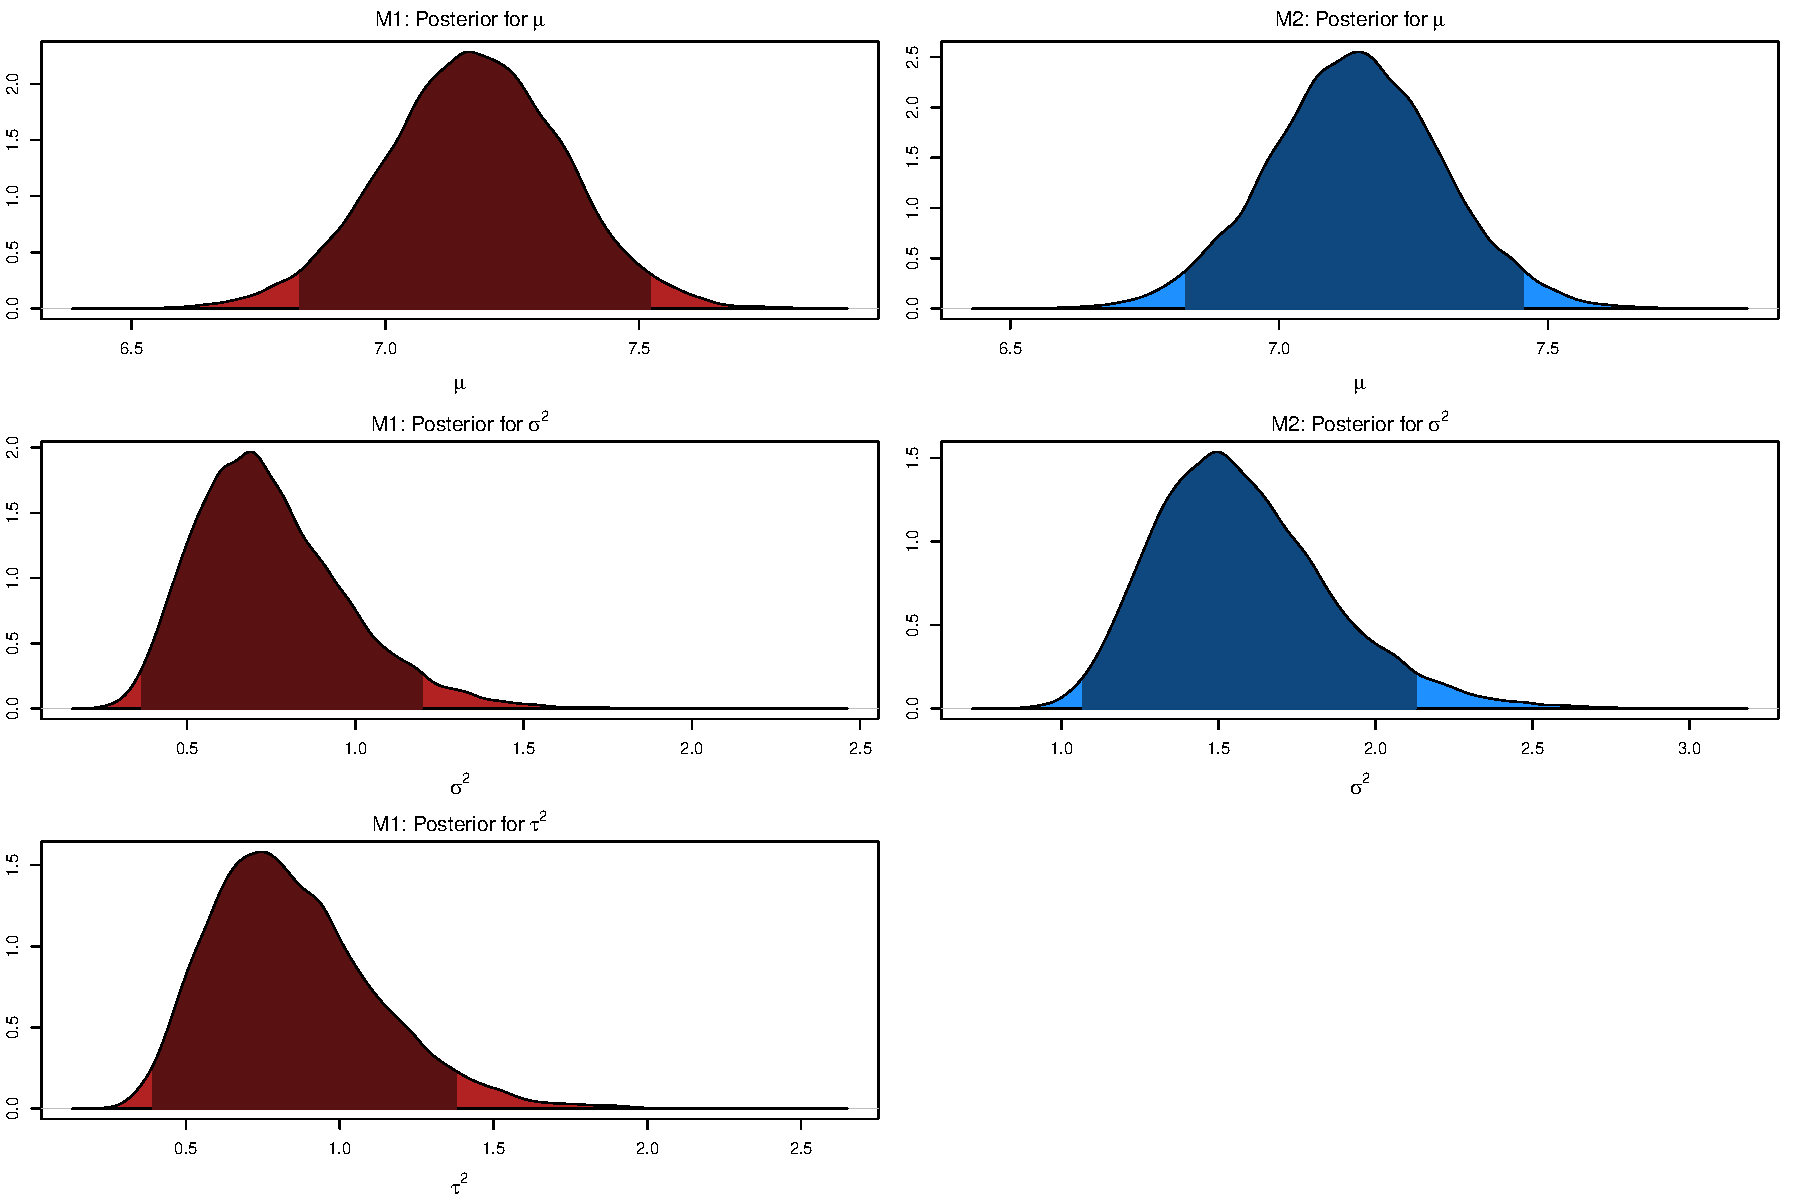
\includegraphics[scale=0.50]{figs/m_post.pdf}
\caption{Posterior distributions from each model. \emph{Left column:} posteriors for $\mu$, $\sigma^2$, and $\tau^2$ in model 1. \emph{Right column}: posteriors for $\mu$ and $\sigma^2$ in model 2. The shaded regions are the HPD regions.}
\label{m_post}
\end{figure*}

If we wish to make a prediction from model 1 for a future observable (one in which we do not know the random effect), we must first draw a new $\mu_0$ from a $N(\mu,\tau^2)$ using the posterior samples for $\mu$ and $\tau^2$. We could then either (1) sample a new $\lambda_0$ from a $Ga(\nu/2,\nu/2)$ and then sample $y_0$ from $N(\mu_0, \sigma^2/\lambda_0)$, or (2) directly sample $y_0$ from $t_\nu(\mu_0, \sigma^2)$. Both approaches are equivalent, and both are very different than predictions made for a particular observation in which the random effect $\mu_i$ is known.

The posterior predictive distribution of a future observation for each model is presented in Figure \ref{post_pred}.

As mentioned in section 2.3.1, the measures of model validation we use are based on posterior predictions. For model 1, we make the calculations based on future observables, not from a particular observation. For the $\chi^2$ test, we use all data points when obtaining posterior samples. The $B$ $p$-values are computed for both models and their distributions are given in Figure \ref{gof}. In both, the probability that the $p$-value is greater than $0.05$ is at least $0.95$, providing evidence the models are appropriate for the data.

The second measure is based on leave-one-out cross-validation. The resulting distributions of probabilities (i.e. the proportion of posterior predictions less than the left-out observation) should be uniformly distributed (see Figure \ref{loo}). A Kolmogorov-Smirnov test is performed on these probabilities and both result in large $p$-values ($0.70$ for model 1 and $0.80$ for model 2). So again, we confirm that the models provide adequate fits to the data.

\begin{figure}
\centering
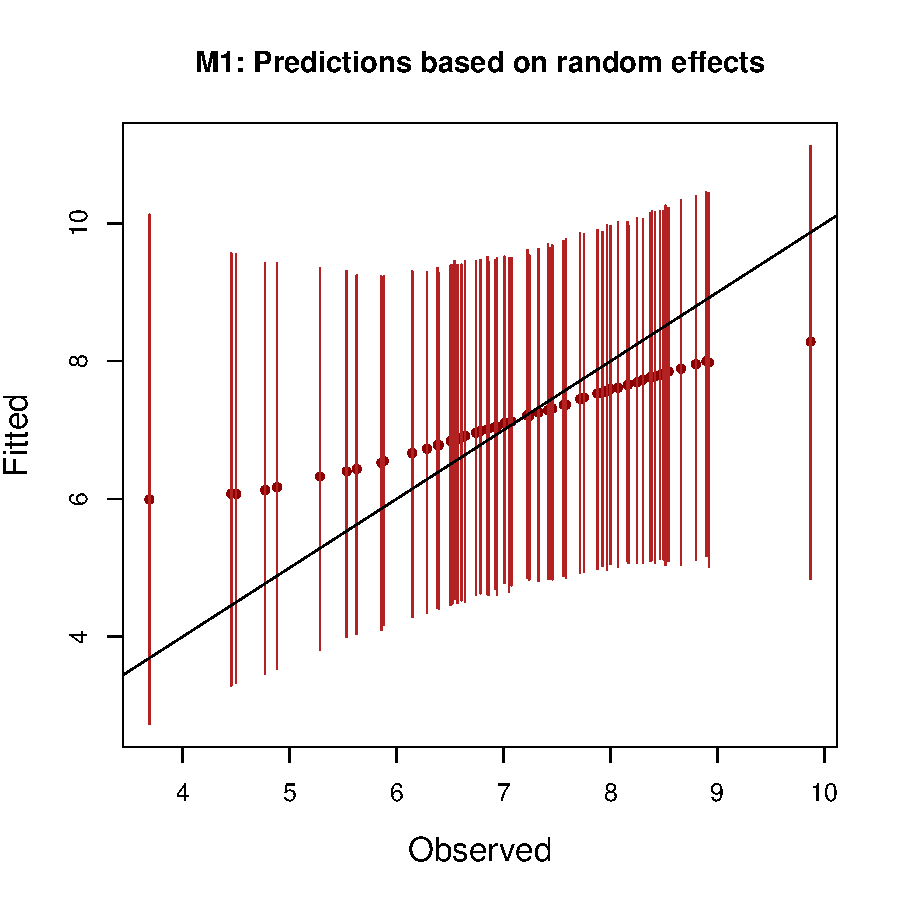
\includegraphics[scale=0.50]{figs/m1_obs_fit.pdf}
\caption{Plot of the observed versus fitted values for individual observations in model 1. The dots are the predictive means and the vertical bars are equal-tailed 95\% probability bounds. The black line is the line $y=x$.}
\label{obs_fit}
\end{figure}

We are now left to question which model is preferred. Based on the evidence so far, both models seem to perform equally well, so we would thus favor the simpler model 2. We can be more certain in our decision as we take a look at the three measures discussed in section 2.3.2. The first two are presented in Table 1. For the posterior predictive loss (PPL) criterion, we decompose the value into the goodness-of-fit term (G) and the penalty (P) to see how the models differ. In both instances (DIC and PPL), the simpler model 2 outperforms the hierarchical model 1.

\begin{table}[h]
\caption{Model comparison quantities}
\centering
\begin{tabular}{lrrrr}
\\ [-5pt]
        & DIC   & G    & P      & PPL(=G+P) \\ \hline
Model 1 & 311.8 & 94.7 & 134.0  & 228.7   \\ 
Model 2 & 205.9 & 94.6 & 99.3   & 194.0   \\ 
   \hline
\end{tabular}
\end{table}

The Bayes factor is estimated using Monte Carlo integration. At one million samples from the prior distribution, we estimate $B_{12}\approx0.623$. Since $B_{12}<1$, this is evidence in favor of model 2, but it is not substantial. All three measures taken together suggest that model 2 is a better choice: it performs just as well as the more complicated model and yet does so with fewer parameters.

\begin{figure}
\centering
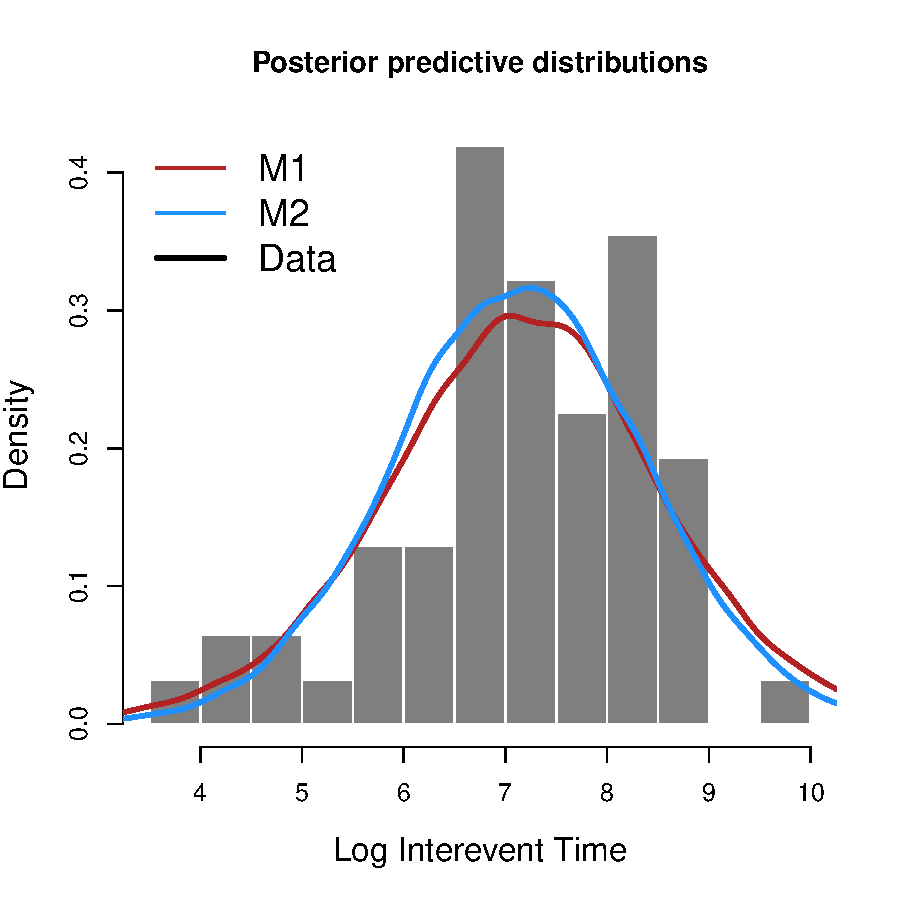
\includegraphics[scale=0.50]{figs/post_pred.pdf}
\caption{Posterior predictive distributions for models 1 (red) and 2 (blue). The histogram is of the data. Predictions for model 1 are based on future observations.}
\label{post_pred}
\end{figure}

\section{Discussion}

In this paper we considered two models for the log of interevent times for Mount Etna eruptions. A hierarchical, student-$t$ model was intended to correctly model any long tails in the data, but we have seen that a simple, two-parameter normal model is adequate.

Both graphical and numerical measures have been used to assess whether the models were an appropriate fit for the data. These are not absolutely decisive, but we found no evidence against the validity of either model.

A comparison was made to see which model performed better. Though they performed about the same, the hierarchical model was penalized far more based on DIC and PPL. All the evidence we have looked at suggest that model 2 is a better candidate for predicting log interevent times.

\begin{figure}
\centering
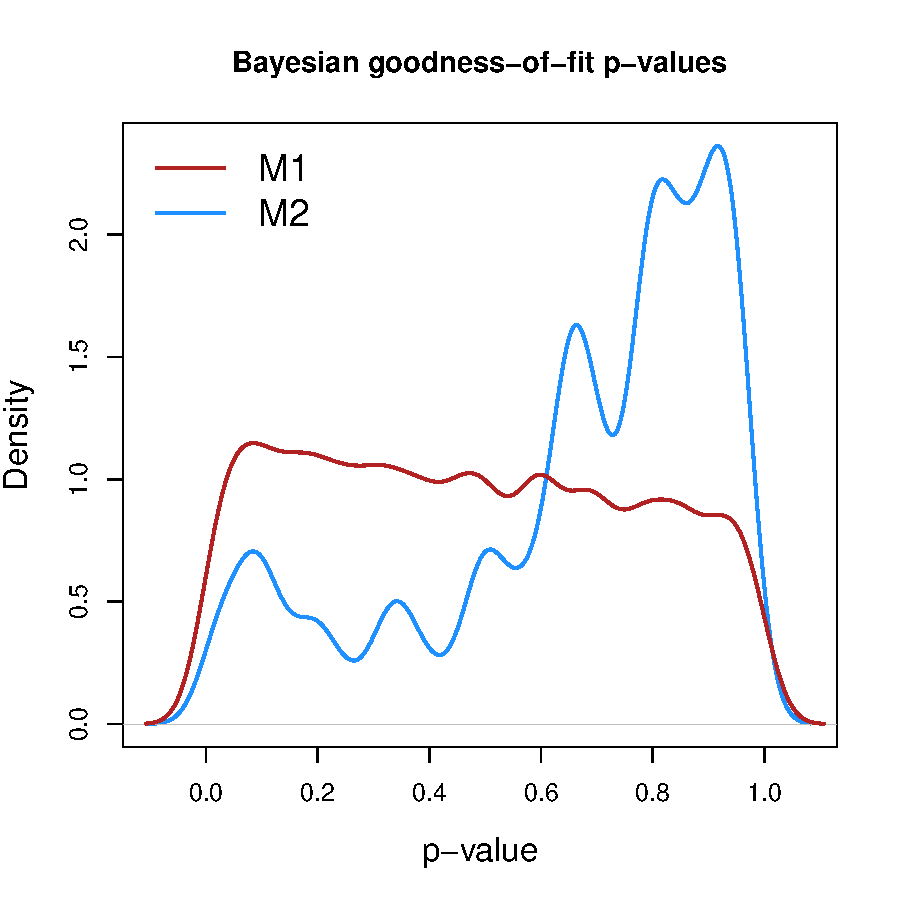
\includegraphics[scale=0.50]{figs/gof.pdf}
\caption{Bayesian goodness-of-fit distribution for $p$-values. \\}
\label{gof}
\end{figure}

\begin{figure}[ht]
\centering
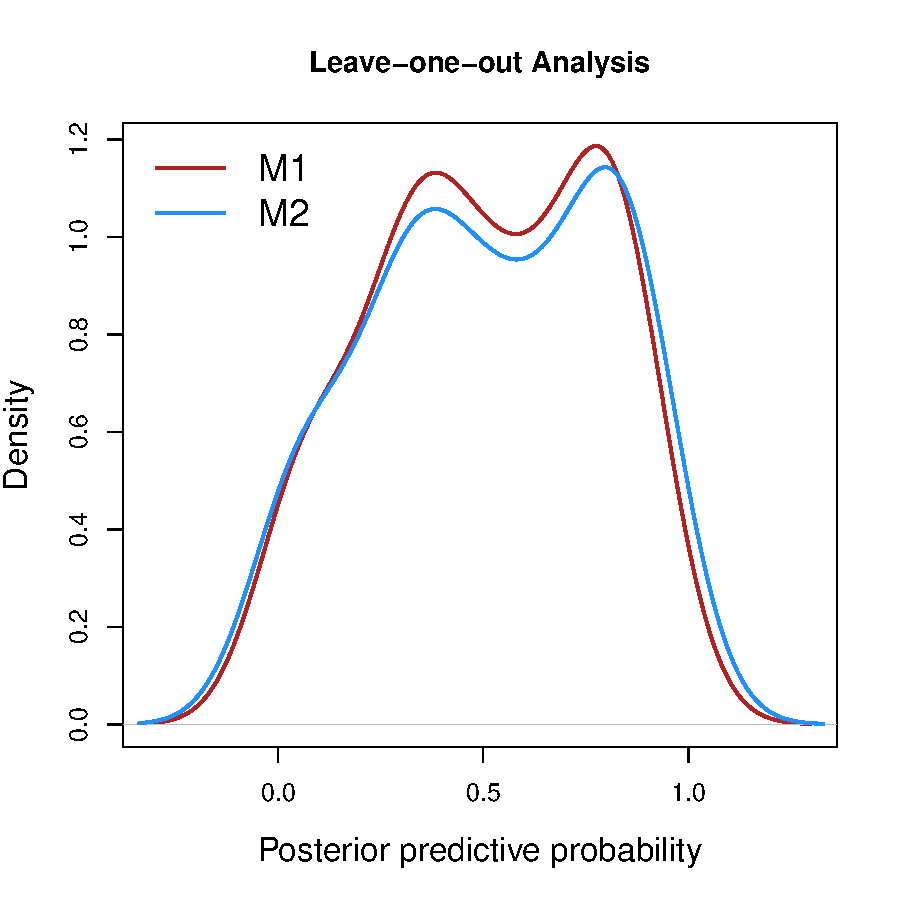
\includegraphics[scale=0.50]{figs/loo.pdf}
\caption{Distributions of the posterior CDF evaluated at each observation.}
\label{loo}
\end{figure}





\end{document}
